% Name: Sierpinski triangle
% Description: The Sierpinski triangle after six steps, drawn as a Lindenmayer system: a triangle with its middle quarter removed, again and again in every corner.
% Tags: Sierpinski triangle, fractal, L-system, self-similarity

\usetikzlibrary{lindenmayersystems}

\pgfdeclarelindenmayersystem{Sierpinski triangle}{
  \symbol{X}{\pgflsystemdrawforward}
  \symbol{Y}{\pgflsystemdrawforward}
  \rule{X -> X-Y+X+Y-X}
  \rule{Y -> YY}}

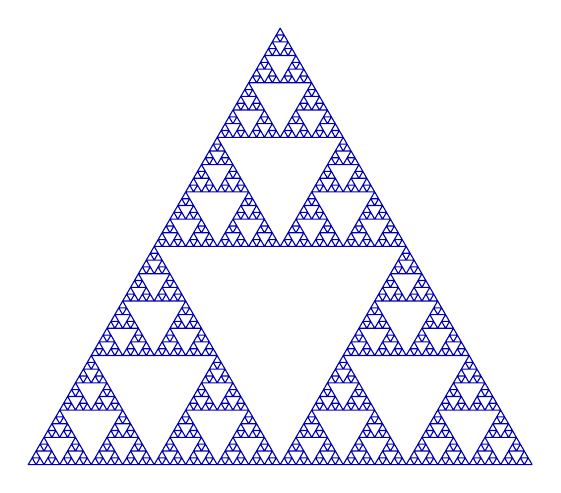
\begin{tikzpicture}
  % Six steps make each side 2⁶ = 64 steps of 1 mm
  \draw[blue!70!black, line join=round, rotate=180, lindenmayer system={Sierpinski triangle, axiom=X-Y-Y, order=6, angle=120, step=1mm}] lindenmayer system;
\end{tikzpicture}
